\documentclass[]{article}


\usepackage{xcolor}
\usepackage[ngerman]{babel}
\usepackage{graphicx}
\usepackage{FiraMono}
\usepackage{mathtools}
\usepackage{cleveref}
\usepackage{titlesec}

\setcounter{secnumdepth}{3}
\setcounter{section}{-1} % This sets the section counter to start at 0


\newcommand{\todo}{\textcolor{red}{TODO}}


%opening
\title{Lernfeld 1 - Das Unternehmen und eigene Rolle im Betrieb}
\author{Alexander Herget}

\begin{document}
	
\maketitle
	
\begin{abstract}

Innerhalb von 11 Thementagen mit je 4 Stunden, die zwischen dem 20.09.2024 und 27.06.2025 stattfinden, soll ich in der Lage sein, das Unternehmen hinsichtlich seiner Wertschöpfungskette zu präsentieren und die eigene Rolle im Betrieb zu beschreiben. \\

Es ist verpflichtend über die Lerneinheiten hinweg ein Portfolio über die Lerninhalte zu führen und es am Ende des Halbjahres zu präsentieren.\\

Zusätzlich zum Portfolio wird am 04.07.2025 die Präsentation durchgeführt und innerhalb eines Team wird es eine multimediale Darstellung meines Unternehmens geplant und erstellt.\\

Als Quellen hierzu dienen der Input von Frau Althans zu verschiedenen Themen, das Miro Board passend zum Lernfeld und die in Moodle zur Verfügung gestellten Materialien.

\end{abstract}

\newpage
\tableofcontents

\newpage	
\section{Thementag 0 - 30.08.2024}

\subsection{Dokumentieren}

Nach einer Recherche die Erkenntnis dokumentieren und niederschreiben. Danach zur restlichen Aufgabe übergehen. Es ist für Schüler verpflichtend ein Portfolio zu führen. Der Zugriff auf die Daten soll jederzeit möglich und teilbar sein. Als positiver Zusatz, wäre es wichtig, zusammen an einem Dokument arbeiten zu können. Es wäre schön, wenn es visualisiert werden kann, da unser Gehirn in Bildern lernt.

Inhaltlich soll ersichtlich sein, wie die Aufgabe lautet und das dazugehörige Infomaterial vorhanden sein, sowie die Ergebnisse und Zwischenergebnisse erkenntlich sein.
	
\section{Thementag 1 - 20.09.2024}

\subsection{Übersicht über das Lernfeld}

Zu Beginn des Thementages gab es eine geforderte Zusammenfassung der Treffen zwischen Klasse und Frau Althans. Danach wurde uns das Miro Board präsentiert und jeder Lernende sollte für sich das Board erkunden. Nach einer gewissen Zeit wurden die verschiedenen Herangehensweisen verglichen und dann geklärt, was die zentralen Fragen eines jeden Lernfelds sind. Als Aufgabe mussten die Lehrenden dann in einem Portfolio übersichtlich auf einer Seite zusammenfassen, was die wichtigen Punkte der Lerneinheit sind/waren. Meine Ergebnisse wurden in der Zusammenfassung nieder geschrieben.

\newpage
\section{Thementag 2 - 11.10.2024}
\subsection{Leitbild und Unternehmenskultur}
\subsubsection{Anspruchsgruppen von Unternehmen}
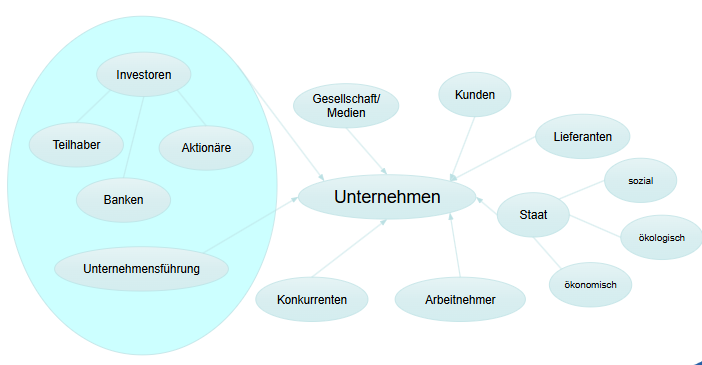
\includegraphics[width=\linewidth]{assetes/Anspruchsgruppen Unternehmen.png}

Unternehmen stehen im ständigen Austausch mit verschiedenen Anspruchsgruppen, die Einfluss auf ihre Entscheidungen und ihr Handeln haben. Diese Gruppen lassen sich grob in interne und externe Gruppen unterteilen. Interne Anspruchsgruppen sind beispielsweise die Unternehmensführung, Teilhaber, Aktionäre, Investoren und Banken. Diese Gruppen befinden sich innerhalb des Unternehmenssystems oder sind direkt an dessen Erfolg beteiligt (z.B. finanziell oder strategisch).

Externe Anspruchsgruppen umfassen unter anderem Kunden, Lieferanten, Arbeitnehmer, den Staat, die Gesellschaft/Medien sowie Konkurrenten. Der Staat hat vielfältige Erwartungen, etwa sozialer, ökologischer oder ökonomischer Natur. Lieferanten beeinflussen die Versorgung mit Gütern und Dienstleistungen, während Kunden über ihr Kaufverhalten den Markterfolg bestimmen. Auch gesellschaftliche Meinungen und Medienberichterstattung wirken sich auf das Unternehmen aus, besonders im Hinblick auf Image und öffentliche Akzeptanz.


\subsubsection{Unternehmenskultur}

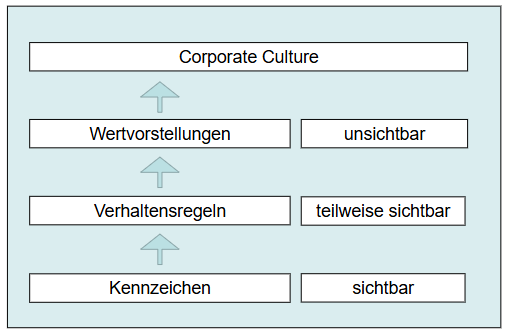
\includegraphics[width=\linewidth*2/3]{assetes/Unternehmeskultur.png}

Die Unternehmenskultur besteht aus mehreren Ebenen: An der Oberfläche stehen sichtbare Kennzeichen wie Kleidung, Sprache oder Rituale. Darunter folgen teilweise sichtbare Verhaltensregeln, etwa im Umgang miteinander oder bei Entscheidungsprozessen. Die tiefste Ebene bilden die unsichtbaren Wertvorstellungen, die grundlegende Überzeugungen und Einstellungen im Unternehmen prägen. Zusammengenommen formen diese Elemente die Unternehmenskultur und beeinflussen maßgeblich das Verhalten und die Identität eines Unternehmens.

\subsubsection{Unternehmensidentität zur Unternehmensphilosophie}

\includegraphics[width=\linewidth*2/3]{assetes/Unternehmesidentität.png}

Die Unternehmensidentität beschreibt das Selbstbild eines Unternehmens und wird systematisch aufgebaut. Der Prozess beginnt mit der Erfassung des aktuellen Unternehmensimage (Fremdbild). Anschließend wird eine Unternehmensphilosophie als Soll-Zustand formuliert. Darauf aufbauend wird ein Maßnahmenkatalog entwickelt und dokumentiert, der konkrete Schritte zur Umsetzung enthält. Abschließend erfolgt die Umsetzung der Maßnahmen sowie eine Erfolgskontrolle, um sicherzustellen, dass die gewünschte Identität erreicht wird.

\subsubsection{Unternehmensleitbild}

Ein Unternehmensleitbild beschreibt die zentralen Ziele, Werte und die grundlegende Ausrichtung eines Unternehmens. Es besteht meist aus Vision (Zukunftsbild), Mission (Auftrag) und den Unternehmenswerten. Das Leitbild dient als Orientierung für Mitarbeitende und Führungskräfte und unterstützt ein einheitliches Auftreten nach innen und außen. Es bildet zudem die Basis für strategische Entscheidungen und die Unternehmenskultur.

\subsubsection{Unternehmensziele}

Unternehmensziele geben die Richtung vor, in die sich ein Unternehmen entwickeln möchte. Sie lassen sich in ökonomische Ziele (z.B. Gewinn, Wachstum, Marktanteil), soziale Ziele (z.B. Mitarbeiterzufriedenheit, Arbeitsbedingungen) und ökologische Ziele (z.B. Umweltschutz, Ressourcenschonung) unterteilen. Ziele helfen dabei, Entscheidungen zu steuern, den Erfolg zu messen und die Motivation der Mitarbeitenden zu stärken. 

\newpage
\section{Thementag 3 - 06.12.2024}

\subsection{Wertschöpfungssystem}

Durch Kombination der Produktionsfaktoren geschaffener Mehrwert in einem Unternehmen. \\

\subsubsection{Produktionsfaktoren}

\begin{enumerate}
	\item Volkswirtschaftliche Produktionsfaktoren\\
	Es gibt 4 Faktoren: Boden, Arbeit, Kapital und Wissen. Zusammen sind die verbundenen Faktoren mehr Wert, schaffen ein Mehrwert. \\
	\begin{itemize}
		\item Boden: Grund, Bodenschätze, Rohstoffe der Natur
		\item Arbeit: die Rohstoffe der Natur zu Gütern umzuwandeln, Arbeit eins einzelnen
		\item Menschen, wird in zwei weitere Kategorien eingeteilt
		\begin{itemize}
			\item Quantität: Anzahl der Mitarbeiter
			\item Qualität: Ausbildungsstand der Mitarbeiter
		\end{itemize}
		\item 	Kapital: wird in zwei Kategorien eingeteilt: Geldkapital und Sachkapital (Gebäude Maschinen und Werkzeuge)
	\end{itemize}
	
	\item Betriebswirtschaftliche Produktionsfaktoren
	\begin{itemize}
		\item Elementarfaktoren
		\begin{itemize}
			\item ausführende Arbeit (fertigen, umsetzen)
			\item Betriebsmittel (Maschinen)
			\item Werkstoffe (Roh, Hilfs- und Betriebsstoffe)
			\item Rechte (Lizenzen, Patente)
		\end{itemize}
		\item dispositiver Faktor (Planung, Steuerung und Kontrolle der Elementarfaktoren)
	\end{itemize}
\end{enumerate}

\subsubsection{Wertschöpfungssystem}
Wertschöpfung ist die Leistung abzüglich der Vorleistung. \\

Als Beispiel verkauft der Bauer an den Müller sein Korn, der mahlt das Mehl und verkauft es an den Bäcker und der letztendlich an den Konsumenten. Der Bauer, Müller und Bäcker bilden hierbei Produktionsstufen um Wertschöpfungssystem.\\
Weil der Staat die Infrastruktur für die Schöpfung des Mehrwert bietet, erhebt der Staat die Mehrwertsteuer und verdient in jeder Produktionsstufe mit. Letztlich werden die Steuerkosten auf den Konsumenten abgewälzt.

\subsubsection{Wertschöpfungssystem im Betrieb}
\includegraphics[width=\linewidth]{assetes/Wertschöpfung im Betrieb.png}


\newpage
\section{Thementag 4 - 15.01.2025}

\subsection{Marktstruktur und Markt}

\subsubsection{Markt}
Markt ist ein \textit{virtueller} Ort des Tausches. Angebot und Nachfrage regeln den Preis. Wenn beides ausgeglichen ist, redet man vom Marktgleichgewicht und es gibt eine Gleichgewichtspreis/menge. 
\subsubsection{Marktarten}
Wenn es keine Regulierung des Markts gibt, dann handelt es sich um einen \textbf{freien Markt}. Dieser existiert nur theoretisch, da es kein Gut unbegrenzt vorhanden ist.\\
Ein Gegenstück zum freien Markt ist der \textbf{begrenzte Markt}. Da Menschen \textit{Präferenzen} (nicht jeder zieht gerne das gleiche an) haben, gibt es \textit{keine unendliche Nachfrage} von \textit{unendlichen Gütern} (Ressourcenknappheit). Dazu gibt es einschränkende \textit{Rechte} und \textit{Verbote}, wie zum Beispiel Patente oder Besitzverbote (Beruhigungsmittel).
\subsubsection{Marktformen}
Es gibt 3 verschiedene begrenzte Märkte: Monopol, Oligopol und Polypol. \\
Beim \textbf{Monopol} füllt ein einziger Anbieter, den Markt alleine mit einem Produkt.\\
Beim \textbf{Oligopol} Auf der Seite des Angebots und/oder der Nachfrage treten wenige relativ große Verkäufer bzw. Käufer auf.\\
Das \textbf{Polypol} ist dazu das Gegenteil zum Monopol, wo es viele Anbieter und Nachfrager gibt.
\subsubsection{Marketing}
Marketing wird auch als \textit{Führen des Unternehmens vom Markt her} definiert. Marketing basiert auf 4 Säulen: Produkt- und Sortimentspolitik, Preispolitik, Absatzpolitik und Kommunikationspolitik.
Die \textbf{Produkt- und Sortimentspolitik} ist das Kernstück des Marketing und umfasst alle Entscheidungen über marktgerechte Gestaltung des Leistungsprogramms. Dabei spielen \textit{Bedürfnisse}, \textit{Wünsche} und \textit{Probleme des Kunden} eine entschiedene Rolle.\\
Die \textbf{Preispolitik} will hauptsächlich Kaufanreize setzen, durch Preisgestaltung.\\
Die \textbf{Absatzpolitik} hat den Fokus auf die Logistik zum Kunden. Alle Maßnahmen, um Absatzleistungen im richtigen Zustand, zum richtigen Zeitpunkt, in gewünschter Menge, am richtigen Ort zur Verfügung zu stellen.\\
Die \textbf{Kommunikationspolitik} übermittelt Informationen zur Steuerung von Meinungen, Einstellungen, Erwartungen und Verhaltensweisen.

\subsubsection{Marktanalyse}
Marktanalyse bildet die Basis allen strategischen Handelns. Dazu werden \textit{Marktbeobachtungen}, \textit{Befragungen} und \textit{Statistiken} durchgeführt. Als Ziel dieser Methoden werden Zielgruppen, Konkurrenz und \textit{Marktanteil} untersucht.
\subsubsection{Marktanteil}
Der \textbf{Marktanteil} ist der eigene Anteil des Marktes am Gesamtmarkt. \\
Der absolute Marktanteil: $\frac{\text{Eigener Absatz (Umsatz)}}{\text{Gesamtabsatz (Umsatz)}} \cdot 100$\\
Der relative Marktanteil: $\frac{\text{Eigener Absatz (Umsatz)}}{\text{Absatz/Umsatz des stärksten Mitbewerbers}} \cdot 100$

\newpage
\section{Thementag 5 - 07.02.2025}

\subsection{Organisationsstruktur}
Organisation kann auf diverse Arten verstanden werden. Es gibt das planmäßige Gestalten von Regelungen, was die Organisation als Tätigkeit definiert. Eine künstlich geschaffene Ordnung ist ein Zustand und die Unternehmung (Unternehmen) selbst ist eine Institution. Im folgenden Input wird er Betrieb im Fokus stehen.

\subsection{Betriebliche Organisation}
Dauerregelungen, sind Regeln die etwas festlegen und dann etwas als nächstes voraussetzen. Als Beispiel gibt es die Regel, dass eine Schule um 8 Uhr startet. Daher wird vorausgesetzt, dass die Schüler bis dahin da sind. Solche Regelungen organisieren den Betrieb und wird als Organisation bezeichnet. \\
Im Gegensatz dazu gibt es die fallweise Regelung. Dort gibt es keine planbare Regel. Bei plötzlich auftretenden Situationen muss sofort gehandelt/\textbf{improvisiert} werden. Wenn im Rahmen einer Dauerregelung eine neue Situation entsteht, dann spricht man von \textbf{Disposition}. Wenn wie im obigen Beispiel jemand zu spät zur Schule kommt, dann tritt eine "Bestrafung" erst nach X Minuten in Kraft.

\subsection{Organisationsgrundsätze}
Es gibt 4 Grundsätze: Klarheit, Zweckmäßigkeit, Wirtschaftlichkeit, Organisatorisches Gleichgewicht.
\begin{itemize}
	\item \textbf{Klarheit} - Regeln müssen eindeutig sein
	\item \textbf{Zweckmäßigkeit} - Angemessene Regelung in Unternehmen
	\item \textbf{Wirtschaftlichkeit} - Ökonomische Prinzipien (Minimum- oder Maximumprinzip)
	\item \textbf{Organisatorisches Gleichgewicht} - Ausgewogenes Verhältnis zwischen Dauerregelungen und fallweisen Regelungen
\end{itemize}

\subsection{Struktur}

\begin{figure}[h]
	\centering
	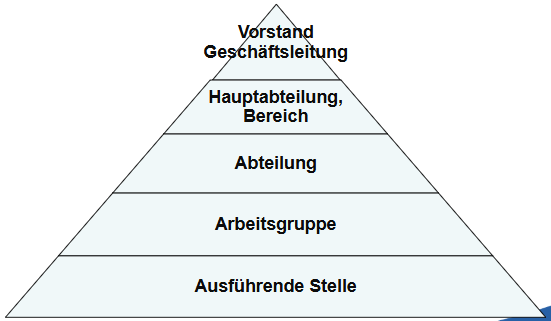
\includegraphics[width=0.7\linewidth]{assetes/Struktur}
	\caption{Betriebliche Struktur}
	\label{fig:struktur}
\end{figure}

\subsection{Organigramme - Einliniensystem}
Linien in einem Organigramm stellen \textbf{Weisungsbefugnis} dar. Das Einliniensystem hat als Vorteil klare Regelungen, ist aber nicht unbedingt wirtschaftlich. Die Kommunikation zwischen Abteilungen kann die Arbeit stark verzögern. 

\begin{figure}[h!]
	\centering
	\includegraphics[width=0.7\linewidth]{"assetes/Organigramm - Einliniensystem"}
	\caption{Einliniensystem}
	\label{fig:organigramm---einliniensystem}
\end{figure}

\subsection{Organigramme - Stabsliniensystem}
Die Stabsstellen haben keine Weisungsbefugnis gegenüber den Abteilungen.
\begin{figure}[h!]
	\centering
	\includegraphics[width=0.7\linewidth]{"assetes/Organigramm - Stabsliniensystem"}
	\caption{Stabsliniensystem}
	\label{fig:organigramm---stabsliniensystem}
\end{figure}


\subsection{Organigramme - Mehrliniensystem}

\begin{figure}[h!]
	\centering
	\includegraphics[width=0.7\linewidth]{"assetes/Organigramm - Mehrliniensystem"}
	\caption{Mehrliniensystem}
	\label{fig:organigramm---mehrliniensystem}
\end{figure}

\subsection{Organigramme - Matrixorganisation}
Die Matrixorganisation kombiniert zwei Mehrliniensysteme.

\begin{figure}[h!]
	\centering
	\includegraphics[width=0.7\linewidth]{"assetes/Organigramm - Matrixorganisation"}
	\caption{Matrixorganisation}
	\label{fig:organigramm---matrixorganisation}
\end{figure}

\subsection{Wichtige Begrifflichkeiten}
\begin{itemize}
	\item Instanz: Weisungsbefugnisebene gegenüber mehreren rangniedrigeren Stellen
	\item Stelle: kleinste, nicht teilbare ausführende Einheit einer Unternehmung 
	\item Abteilung: organisatorische Zusammenfassung von einzelnen Stellen zu einer Einheit, die eine spezialisierte Tätigkeit ausführt
	\item Stabsstelle: ist einer Instanz untergestellt, hat jedoch keine Weisungsbefugnisse; Hilfs- und Beratungsfunktion
\end{itemize}

\newpage
\section{Thementag 6 - 28.02.2025}
Rechtsformen beziehen sich auf die Art von Unternehmen. Für die Präsentation des eigenen Unternehmens genügt eine Erwähnung. In der Abschlussprüfung gibt es sowohl im WiSo Teil, als auch in den freien Fragen, spielen Rechtsformen eine entschiedene Rolle.

\subsection{Rechtsformen im Überblick}

Das Handelsgesetzbuch schreibt den Rechtsformen verschiedene Rahmenbedingungen gegenüber dem Gesetz vor. Jede Rechtsform hat Vor- und Nachteile und muss je nach Situation und Zielen abgewogen werden.

\begin{figure}[h!]
	\centering
	\includegraphics[width=0.7\linewidth]{"assetes/Rechtsform"}
	\caption{Rechtsformen Überblick}
	\label{fig:rechtsformen---rechtsformenüberblick}
\end{figure}

\subsection{Gründe für eine Wahl einer Rechtsform}

Es gibt ein paar Leitfragen für die Wahl der Rechtsform:

\begin{itemize}
	\item Ist ein Partner vorhanden?
	\item Wer soll „das Sagen“ im Unternehmen haben?
	\item Wie gut sind die Finanzierungsmöglichkeiten
	\item Wie soll der Gewinn verteilt werden?
	\item Wer haftet in welchem Umfang?
\end{itemize}



\subsection{Personen im Rechtsverkehr}

\begin{minipage}[t]{0.45\textwidth}
	natürliche Personen
	\begin{itemize}
		\item alle Menschen ohne Rücksicht auf Alter, Geschlecht und Rasse
	\end{itemize}
\end{minipage}
\hfill
\begin{minipage}[t]{0.45\textwidth}
	juristische Personen
	\begin{itemize}
		\item für das Recht fiktiv geschaffene Personen
		\item Personenvereinigungen
		\item Vermögensmassen mit eigener Rechtspersönlichkeit
	\end{itemize}
\end{minipage}

\subsection{Rechtsfähigkeit}

\begin{minipage}[t]{0.45\textwidth}
	natürliche Personen
	\begin{itemize}
		\item Alle Personen sind mit Vollendung der Geburt bis zum Tod (§ 1 BGB) rechtsfähig
		\item d.h. haben alle gesetzlichen Rechte und Pflichten
	\end{itemize}
\end{minipage}
\hfill
\begin{minipage}[t]{0.45\textwidth}
	juristische Personen
	\begin{itemize}
		\item Beginnt mit der Eintragung in	das jeweilige Register und endet mit der Löschung in diesem Register
		\item und haben dann ebenfalls alle gesetzlichen Rechte und Pflichten
	\end{itemize}
\end{minipage}

\newpage
\subsection{Rechtsformen im Überblick und Erläuterung}

Umsatzsteuerstatistik aus 2005, aber heute noch sehr ähnlich.

\begin{tabular}{|c|c|c|}
	\hline
	Rechtsformen & Steuerpflichtige Betriebe in \% & Steuerpflichtiger Umsatz in \% \\
	\hline
	Einzelunternehmen & 70,2 & 10,8 \\
	\hline
	OHG (incl. GBR) & 8,6 & 5,0 \\
	\hline
	KG (incl. GmbH \& Co KG) & 4,0 & 23,4 \\
	\hline
	AG (incl. KGaA) & 0,2 & 19,6 \\
	\hline
	GmbH & 14,9 & 34,6 \\
	\hline
\end{tabular}

\subsubsection{Einzelunternehmung}
\textbf{Merkmal}: Eine \textit{natürliche Person} ist alleiniger Inhaber des Unternehmens.

\begin{minipage}[t]{0.45\textwidth}
	Vorteile:
	\begin{itemize}
		\item kein vorgeschr. Unternehmenskapital
		\item keine Gewinnverteilung
		\item alleinige Geschäftsleitung
		\item hohe Flexibilität
		\item Kleingewerbebetreibung
		\item Gründung formlos und günstig
	\end{itemize}
\end{minipage}
\hfill
\begin{minipage}[t]{0.45\textwidth}
	Nachteile
	\begin{itemize}
		\item volle Verantwortung
		\item volles Risiko
		\item beschr. Kapitalbeschaffung
		\item i.d.R. hohe Arbeitsbelastung
		\item private Haftung in vollem Umfang
	\end{itemize}
\end{minipage}

\subsubsection{Gesellschaft bürgerlichen Rechts}
\textbf{Merkmal}: Gründung einer \textit{Personengesellschaft} durch (formlosen) Vertragsabschluss mindestens 2er Personen mit gemeinsamen Ziel.

\begin{minipage}[t]{0.45\textwidth}
	Vorteile:
	\begin{itemize}
		\item Keine Eintragung ins HR
		\item Kein vorgeschriebenes Mindestkapital
		\item Beteiligung aller Gesellschafter
	\end{itemize}
\end{minipage}
\hfill
\begin{minipage}[t]{0.45\textwidth}
	Nachteile
	\begin{itemize}
		\item gesamtschuldnerische Haftung aller Gesellschafter auch mit Privatvermögen
		\item Interne Auseinandersetzungen können schnell existenzgefährdend sein
	\end{itemize}
\end{minipage}

\newpage
\subsubsection{Offene Handelsgesellschaft (OHG)}
\textbf{Merkmal}: \textit{Personengesellschaft} von Kaufleuten mit dem Zweck ein bestimmtes Gewerbe unter gemeinsamen Namen zu betreiben. Bei der Gründung muss eine Eintragung im Handelsregister erfolgen.

\begin{minipage}[t]{0.45\textwidth}
	Vorteile:
	\begin{itemize}
		\item kein vorgeschriebenes Mindestkapital
		\item höhere Kreditwürdigkeit
		\item jeder Gesellschafter besitzt Geschäftsführungsmöglichkeit
	\end{itemize}
\end{minipage}
\hfill
\begin{minipage}[t]{0.45\textwidth}
	Nachteile
	\begin{itemize}
		\item gesamtschuldnerische Haftung der Gesellschafter mit Privatvermögen
		\item hohes Maß an Vertrauen notwendig
		\item interne Auseinandersetzungen können Existenz gefährden
	\end{itemize}
\end{minipage}

\subsubsection{Kommanditgesellschaft (KG)}
\textbf{Merkmal}: 2 Arten von Gesellschaftern bei folgender \textit{Personengesellschaft}:
\begin{itemize}
	\item Komplementär (Vollhafter – wie OHG Gesellschafter)
	\item Kommanditist (Teilhafter)
\end{itemize}

\begin{minipage}[t]{0.45\textwidth}
	Vorteile:
	\begin{itemize}
		\item nur Komplementär(Geschäftsführer) haftet persönlich und gesamtschuldnerisch
	\end{itemize}
\end{minipage}
\hfill
\begin{minipage}[t]{0.45\textwidth}
	Nachteile
	\begin{itemize}
		\item Pflichteinlage der Kommanditisten
		\item Kommanditist besitzt keine Geschäftsführungsberechtigung
		\item Eintragungen in Handelsregister erforderlich
	\end{itemize}
\end{minipage}

\subsubsection{Gesellschaft mit beschränkter Haftung (GmbH)}
\textbf{Merkmal}: Gründung eine \textit{Kapitalgesellschaft} durch ein oder mehrere Gesellschafter

\begin{minipage}[t]{0.45\textwidth}
	Vorteile:
	\begin{itemize}
		\item begrenzte Haftung
		\item Trennung Inhaberschaft und Geschäftsführung möglich
		\item Haftung nur mit dem Geschäftsvermögen 
	\end{itemize}
\end{minipage}
\hfill
\begin{minipage}[t]{0.45\textwidth}
	Nachteile
	\begin{itemize}
		\item Stammkapital 25.000€
		\item aufwändige Gründung (Notar, HR)
		\item Kapitalbeschaffung schwieriger
	\end{itemize}
\end{minipage}

\subsubsection{Unternehmergesellschaft (UG)}
\textbf{Merkmal}: Gründung eine \textit{Kapitalgesellschaft} durch ein oder mehrere Gesellschafter

\begin{minipage}[t]{0.45\textwidth}
	Vorteile:
	\begin{itemize}
		\item begrenzte Haftung
		\item Stammkapital mindestens 1€
		\item Trennung Inhaberschaft und Geschäftsführung möglich
		\item Haftung nur mit dem Geschäftsvermögen 
	\end{itemize}
\end{minipage}
\hfill
\begin{minipage}[t]{0.45\textwidth}
	Nachteile
	\begin{itemize}
		\item aufwändige Gründung (Notar, HR)
		\item Kapitalbeschaffung noch schwieriger
		\item gesetzliche Verpflichtung zur Rücklage von 1/3 des Gewinns
	\end{itemize}
\end{minipage}

\subsubsection{Aktiengesellschaft (AG)}
\textbf{Merkmale}: 
\begin{itemize}
	\item Grundkapital (gezeichnetes Kapital) ist in Aktien zerlegt
	\item Organisation
	\begin{itemize}
		\item Vorstand: Geschäftsführungsorgan
		\item Aufsichtsrat: Kontrollorgan
		\item Hauptversammlung: Alle Mitglieder/Teilhaber
	\end{itemize}
\end{itemize}

\begin{minipage}[t]{0.45\textwidth}
	Vorteile:
	\begin{itemize}
		\item Haftung nur mit Geschäftsvermögen
		\item einfache Beschaffung von EK möglich
		\item hohe Kreditwürdigkeit
		\item Unternehmenskontinuität 
	\end{itemize}
\end{minipage}
\hfill
\begin{minipage}[t]{0.45\textwidth}
	Nachteile
	\begin{itemize}
		\item Vorgeschriebenes Stammkapital 50.000€
		\item aufwändige Entscheidungsprozesse aufgrund der straffen Organisation
		\item hoher Finanzaufwand zur Gründung
		\item hoher organisatorischer Aufwand
	\end{itemize}
\end{minipage}

\newpage
\subsubsection{Sonderform GmbH \& Co. KG}
Eigentliche Rechtsform ist KG:

\begin{figure}[h!]
	\centering
	\includegraphics[width=0.7\linewidth]{"assetes/GmbH und Co KG"}
	\caption{GmbH \& Co. KG}
	\label{fig:rechtsformen---gmbh_cokg}
\end{figure}

\newpage
\subsection{Eigener Handlungs- und Entscheidungsspielraum}

In Unternehmen ist es ab einer gewissen Größe notwendig die Entscheidungsträger zu verteilen. Es gibt mehrere Möglichkeiten dies umzusetzen. Zum Beispiel mit Team- bzw. Abteilungsleiter, welche für den jeweiligen Themenbereich vollständige Entscheidungsgewalt inne haben. Die Unternehmensführung vertraut den Entscheidungen und trägt diese mit. Bei einem traditionelleren Unternehmensstruktur, wo Team- oder Abteilungsleiter keine Entscheidungsgewalt haben, kann auf zwei Arten ein Teil der Entscheidungsgewalt übertragen werden.

\subsubsection{Prokura}
Die Prokura ist die höchste Form jemanden Entscheidungsgewalt im Unternehmen zu übertragen. Als Prokurist hat man fast uneingeschränkte Handlungsvollmacht. Es handelt sich hierbei um eine \textit{ausdrückliche Erteilung} von Entscheidungsgewalt und bei Erteilung muss das ins Handelsregister eingetragen werden. Prokura können nur Kaufleute im Sinne des Handelsgesetzbuches erteilen.
Als Prokurist ist man ermächtigt alle gerichtlichen und außergerichtlichen Geschäften und Rechtshandlungen, die der Betrieb des Handelsgewerbes mit sich bringt.
Es gibt verschiedene Arten von Prokura:
\begin{itemize}
	\item Einzelprokura
	\begin{itemize}
		\item Ein einziger Mensch hält die vollkommene Entscheidungsgewalt
	\end{itemize}
	\item Gesamtprokura
	\begin{itemize}
		\item Zwei oder mehrere Prokuristen
		\item Können nur zusammen entscheiden
		\item müssen sich absprechen $\rightarrow$ Kontrollmechanismus
		\item eine Person nicht überlasten
	\end{itemize}
	\item Filialprokura 
	\begin{itemize}
		\item Uneingeschränkte Handlungsfähigkeit für die Filiale
		\item nicht auf das gesamte Unternehmen bezogen
	\end{itemize}
\end{itemize}

Als Prokurist hat man nicht die gleiche Handlungsfähigkeit, wie der Unternehmenseigner. Er darf nicht
\begin{itemize}
	\item Bilanzen/Steuererklärungen unterschreiben
	\item Prokura erteilen
	\item Eintragungen im Handelsregister vornehmen lassen
	\item Insolvenz beantragen
	\item im Sinne des Unternehmens einen Eid leisten
	\item Gesellschafter aufnehmen
	\item Geschäft auflösen oder verkaufen
\end{itemize}

Wenn man als Prokurist unterschreibt, muss das Kürzel PPA vorhanden sein.

\subsubsection{Handlungsvollmacht}
Eine solche Vollmacht kann man mündlich, schriftlich oder durch stillschweigen aussprechen. Diese muss nicht im Handelsregister eingetragen werden. Die Handlungsvollmacht muss nicht vom Unternehmenseigner ausgesprochen werden, sondern auch vom Prokuristen oder auch von einem Vorgesetzten. Die Bevollmächtigung erstreckt sich auf branchenübliche Rechtsgeschäfte. Es gibt verschiedene Arten von Handlungsvollmachten:
\begin{itemize}
	\item Allgemeine Handlungsvollmacht
	\begin{itemize}
		\item übliche Rechtsgeschäfte
	\end{itemize}
	\item Artvollmacht
	\begin{itemize}
		\item Bestimmte Art von Rechtsgeschäften
		\item z.B. Verkauf/Einkauf
	\end{itemize}
	\item Einzelvollmacht
	\begin{itemize}
		\item einmalige Ausübung eines einzelnen Rechtsgeschäft
	\end{itemize}
\end{itemize}

Ohne Sondervollmacht sind nur gewöhnliche Rechtsgeschäfte möglich. Mit Sondervollmacht:
\begin{itemize}
	\item Aufnahme von Darlehen
	\item Grundstückskauf/-verkauf/-belastung
	\item Wechselunterschrift
	\item Prozessführung
\end{itemize}

Wenn man mit Vollmacht unterschreibt, muss das Kürzel i.V. vorhanden sein.



\end{document}
